\section{Composite widgets and alert
dialog}\label{composite-widgets-and-alert-dialog}

The source files are in the
\href{https://github.com/ToshioCP/Gtk4-tutorial}{Gtk4 tutorial GitHub
repository}. Download it and see \passthrough{\lstinline!src/tfe6!}
directory.

\subsection{An outline of new Tfe text
editor}\label{an-outline-of-new-tfe-text-editor}

Tfe text editor will be restructured. The program is divided into six
parts.

\begin{itemize}
\tightlist
\item
  Main program: the C main function.
\item
  TfeApplication object: It is like GtkApplication but keeps GSettings
  and CSS Provider.
\item
  TfeWindow object: It is a window with buttons and a notebook.
\item
  TfePref object: A preference dialog.
\item
  TfeAlert object: An alert dialog.
\item
  pdf2css.h and pdf2css.c: Font and CSS utility functions.
\end{itemize}

This section describes TfeAlert. Others will be explained in the
following sections.

\subsection{Composite widgets}\label{composite-widgets}

The alert dialog is like this:

\begin{figure}
\centering
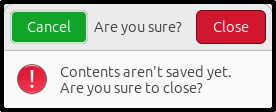
\includegraphics[width=4.2cm,height=1.7cm]{../image/alert.png}
\caption{Alert dialog}
\end{figure}

Tfe uses it when a user quits the application or closes a notebook
without saving data to files.

The dialog has a title, buttons, an icon and a message. Therefore, it
consists of several widgets. Such dialog is called a composite widget.

Composite widgets are defined with template XMLs. The class is built in
the class initialization function and the instances are built and
desposed by the following functions.

\begin{itemize}
\tightlist
\item
  gtk\_widget\_init\_template
\item
  gtk\_widget\_dispose\_template
\end{itemize}

TfeAlert is a good example to know composite widgets. It is defined with
the three files.

\begin{itemize}
\tightlist
\item
  tfealert.ui: XML file
\item
  tfealert.h: Header file
\item
  tfealert.c: C program file
\end{itemize}

\subsection{The XML file}\label{the-xml-file}

A template tag is used in a composite widget XML.

\begin{lstlisting}[language=XML, numbers=left]
<?xml version="1.0" encoding="UTF-8"?>
<interface>
  <template class="TfeAlert" parent="GtkWindow">
    <property name="resizable">FALSE</property>
    <property name="modal">TRUE</property>
    <property name="titlebar">
      <object class="GtkHeaderBar">
        <property name="show-title-buttons">FALSE</property>
        <property name="title-widget">
          <object class="GtkLabel" id="lb_title">
            <property name="label">Are you sure?</property>
            <property name="single-line-mode">True</property>
          </object>
        </property>
        <child type="start">
          <object class="GtkButton" id="btn_cancel">
            <property name="label">Cancel</property>
            <style>
              <class name="suggested-action"/>
            </style>
            <signal name="clicked" handler="cancel_cb" swapped="TRUE" object="TfeAlert"></signal>
          </object>
        </child>
        <child type="end">
          <object class="GtkButton" id="btn_accept">
            <property name="label">Close</property>
            <style>
              <class name="destructive-action"/>
            </style>
            <signal name="clicked" handler="accept_cb" swapped="TRUE" object="TfeAlert"></signal>
          </object>
        </child>
      </object>
    </property>
    <child>
      <object class="GtkBox">
        <property name="orientation">GTK_ORIENTATION_HORIZONTAL</property>
        <property name="spacing">12</property>
        <property name="margin-top">12</property>
        <property name="margin-bottom">12</property>
        <property name="margin-start">12</property>
        <property name="margin-end">12</property>
        <child>
          <object class="GtkImage">
            <property name="icon-name">dialog-warning</property>
            <property name="icon-size">GTK_ICON_SIZE_LARGE</property>
          </object>
        </child>
        <child>
          <object class="GtkLabel" id="lb_message">
          </object>
        </child>
      </object>
    </child>
  </template>
</interface>
\end{lstlisting}

\begin{itemize}
\tightlist
\item
  3: A template tag defines a composite widget. The class attribute
  tells the class name of the composite widget. The parent attribute
  tells the parent class of the composite widget. So, TfeAlert is a
  child class of GtkWindow. A parent attribute is an option and you can
  leave it out. But it is recommended to write it in the template tag.
\item
  4-6: Its three properties are defined. These properties are inherited
  from GtkWindow. The titlebar property has a widget for a custom title
  bar. The typical widget is GtkHeaderBar.
\item
  8: If the property ``show-title-buttons'' is TRUE, the title buttons
  like close, minimize and maximize are shown. Otherwise it is not
  shown. The TfeAlert object is not resizable. It is closed when either
  of the two buttons, cancel or accept, is clicked. Therefore the title
  buttons are not necessary and this property is set to FALSE.
\item
  9-14: The bar has a title, which is a GtkLabel widget. The default
  title is ``Are you sure?'' but it can be replaced by an instance
  method.
\item
  15-32: The bar has two buttons, cancel and accept. The cancel button
  is on the left so the child tag has
  \passthrough{\lstinline!type="start"!} attribute. The accept button is
  on the right so the child tag has \passthrough{\lstinline!type="end"!}
  attribute. The dialog is shown when the user clicked the close button
  or the quit menu without saving the data. Therefore, it is safer for
  the user to click on the cancel button of the alert dialog. So, the
  cancel button has a ``suggested-action'' CSS class. Ubuntu colors the
  button green but the color can be blue or other appropriate one
  defined by the system. In the same way the accept button has a
  ``destructive-action'' CSS class and is colored red. Two buttons have
  signals which are defined by the signal tags.
\item
  35-54: A horizontal box has an image icon and a label.
\item
  44-47: The GtkImage widget displays an image. The ``icon-name''
  property is an icon name in the icon theme. The theme depends on your
  system. You can check it with an icon browser.
\end{itemize}

\begin{lstlisting}
$ gtk4-icon-browser
\end{lstlisting}

The ``dialog-warning'' icon is something like this.

\begin{figure}
\centering

\includegraphics[width=4.19cm,height=1.62cm]{../image/dialog_warning.png}
\caption{dialog-warning icon is like \ldots{}}
\end{figure}

These are made by my hand. The real image on the alert dialog is nicer.

It is possible to define the alert widget as a child of GtkDialog. But
GtkDialog is deprecated since GTK version 4.10. And users should use
GtkWindow instead of GtkDialog.

\subsection{The header file}\label{the-header-file}

The header file is similar to the one of TfeTextView.

\begin{lstlisting}[language=C, numbers=left]
#pragma once

#include <gtk/gtk.h>

#define TFE_TYPE_ALERT tfe_alert_get_type ()
G_DECLARE_FINAL_TYPE (TfeAlert, tfe_alert, TFE, ALERT, GtkWindow)

/* "response" signal id */
enum TfeAlertResponseType
{
  TFE_ALERT_RESPONSE_ACCEPT,
  TFE_ALERT_RESPONSE_CANCEL
};

const char *
tfe_alert_get_title (TfeAlert *alert);

const char *
tfe_alert_get_message (TfeAlert *alert);

const char *
tfe_alert_get_button_label (TfeAlert *alert);

void
tfe_alert_set_title (TfeAlert *alert, const char *title);

void
tfe_alert_set_message (TfeAlert *alert, const char *message);

void
tfe_alert_set_button_label (TfeAlert *alert, const char *btn_label);

GtkWidget *
tfe_alert_new (void);

GtkWidget *
tfe_alert_new_with_data (const char *title, const char *message, const char* btn_label);
\end{lstlisting}

\begin{itemize}
\tightlist
\item
  5-6: These two lines are always needed to define a new object.
  \passthrough{\lstinline!TFE\_TYPE\_ALERT!} is the type of TfeAlert
  object and it is a macro expanded into
  \passthrough{\lstinline!tfe\_alert\_get\_type ()!}.
  G\_DECLARE\_FINAL\_TYPE macro is expanded into:

  \begin{itemize}
  \tightlist
  \item
    The declaration of the function
    \passthrough{\lstinline!tfe\_alert\_get\_type!}
  \item
    \passthrough{\lstinline!TfeAlert!} is defined as a typedef of
    \passthrough{\lstinline!struct \_TfeAlert!}, which is defined in the
    C file.
  \item
    \passthrough{\lstinline!TFE\_ALERT!} and
    \passthrough{\lstinline!TFE\_IS\_ALERT!} macro is defined as a cast
    and type check function.
  \item
    \passthrough{\lstinline!TfeAlertClass!} structure is defined as a
    final class.
  \end{itemize}
\item
  8-13: The TfeAlert class has a ``response'' signal. It has a parameter
  and the parameter type is defined as a
  \passthrough{\lstinline!TfeAlertResponseType!} enumerative constant.
\item
  15-31: Getter and setter methods.
\item
  33-37: Functions to create a instance. The function
  \passthrough{\lstinline!tfe\_alert\_new\_with\_data!} is a convenience
  function, which creates an instance and sets data at once.
\end{itemize}

\subsection{The C file}\label{the-c-file}

\subsubsection{Functions for composite
widgets}\label{functions-for-composite-widgets}

The following codes are extracted from
\passthrough{\lstinline!tfealert.c!}.

\begin{lstlisting}[language=C]
#include <gtk/gtk.h>
#include "tfealert.h"

struct _TfeAlert {
  GtkWindow parent;
  GtkLabel *lb_title;
  GtkLabel *lb_message;
  GtkButton *btn_accept;
  GtkButton *btn_cancel;
};

G_DEFINE_FINAL_TYPE (TfeAlert, tfe_alert, GTK_TYPE_WINDOW);

static void
cancel_cb (TfeAlert *alert) {
  ... ... ...
}

static void
accept_cb (TfeAlert *alert) {
  ... ... ...
}

static void
tfe_alert_dispose (GObject *gobject) { // gobject is actually a TfeAlert instance.
  gtk_widget_dispose_template (GTK_WIDGET (gobject), TFE_TYPE_ALERT);
  G_OBJECT_CLASS (tfe_alert_parent_class)->dispose (gobject);
}

static void
tfe_alert_init (TfeAlert *alert) {
  gtk_widget_init_template (GTK_WIDGET (alert));
}

static void
tfe_alert_class_init (TfeAlertClass *class) {
  G_OBJECT_CLASS (class)->dispose = tfe_alert_dispose;
  gtk_widget_class_set_template_from_resource (GTK_WIDGET_CLASS (class), "/com/github/ToshioCP/tfe/tfealert.ui");
  gtk_widget_class_bind_template_child (GTK_WIDGET_CLASS (class), TfeAlert, lb_title);
  gtk_widget_class_bind_template_child (GTK_WIDGET_CLASS (class), TfeAlert, lb_message);
  gtk_widget_class_bind_template_child (GTK_WIDGET_CLASS (class), TfeAlert, btn_accept);
  gtk_widget_class_bind_template_child (GTK_WIDGET_CLASS (class), TfeAlert, btn_cancel);
  gtk_widget_class_bind_template_callback (GTK_WIDGET_CLASS (class), cancel_cb);
  gtk_widget_class_bind_template_callback (GTK_WIDGET_CLASS (class), accept_cb);
  ... ... ...
}

GtkWidget *
tfe_alert_new (void) {
  return GTK_WIDGET (g_object_new (TFE_TYPE_ALERT, NULL));
}
\end{lstlisting}

\begin{itemize}
\tightlist
\item
  The macro \passthrough{\lstinline!G\_DEFINE\_FINAL\_TYPE!} is
  available since GLib version 2.70. It is used only for a final type
  class. You can use \passthrough{\lstinline!G\_DEFINE\_TYPE!} macro
  instead. They are expanded into:

  \begin{itemize}
  \tightlist
  \item
    The declaration of the functions
    \passthrough{\lstinline!tfe\_alert\_init!} and
    \passthrough{\lstinline!tfe\_alert\_class\_init!}. They are defined
    in the following part of the C program.
  \item
    The definition of the variable
    \passthrough{\lstinline!tfe\_alert\_parent\_class!}.
  \item
    The definition of the function
    \passthrough{\lstinline!tfe\_alert\_get\_type!}.
  \end{itemize}
\item
  The names of the members of \passthrough{\lstinline!\_TfeAlert!},
  which are \passthrough{\lstinline!lb\_title!},
  \passthrough{\lstinline!lb\_message!},
  \passthrough{\lstinline!btn\_accept!} and
  \passthrough{\lstinline!btn\_cancel!}, must be the same as the id
  attribute in the XML file \passthrough{\lstinline!tfealert.ui!}.
\item
  The function \passthrough{\lstinline!tfe\_alert\_class\_init!}
  initializes the composite widget class.

  \begin{itemize}
  \tightlist
  \item
    The function
    \passthrough{\lstinline!gtk\_widget\_class\_set\_template\_from\_resource!}
    sets the template of the class. The template is built from the XML
    resource ``tfealert.ui''. At this moment no instance is created. It
    just makes the class recognize the structure of the object. That's
    why the top level tag is not object but template in the XML file.
  \item
    The function macro
    \passthrough{\lstinline!gtk\_widget\_class\_bind\_template\_child!}
    connects the member of TfeAlert and the object class in the
    template. So, for example, you can access to
    \passthrough{\lstinline!lb\_title!} GtkLabel instance via
    \passthrough{\lstinline!alert->lb\_title!} where
    \passthrough{\lstinline!alert!} is an instance of TfeAlert class.
  \item
    The function
    \passthrough{\lstinline!gtk\_widget\_class\_bind\_template\_callback!}
    connects the callback function and the
    \passthrough{\lstinline!handler!} attribute of the signal tag in the
    XML. For example, the ``clicked'' signal on the cancel button has a
    handler named ``cancel\_cb'' in the signal tag. And the function
    \passthrough{\lstinline!cancel\_cb!} exists in the C file above.
    These two are connected so when the signal is emitted the function
    \passthrough{\lstinline!cancel\_cb!} is called. You can add
    \passthrough{\lstinline!static!} storage class to the callback
    function thanks to this connection.
  \end{itemize}
\item
  The function \passthrough{\lstinline!tfe\_alert\_init!} initializes
  the newly created instance. You need to call
  \passthrough{\lstinline!gtk\_widget\_init\_template!} to create and
  initialize the child widgets in the template.
\item
  The function \passthrough{\lstinline!tfe\_alert\_despose!} releases
  objects. The function
  \passthrough{\lstinline!gtk\_widget\_despose\_template!} clears the
  template children.
\item
  The function \passthrough{\lstinline!tfe\_alert\_new!} creates the
  composite widget TfeAlert instance. It creates not only TfeAlert
  itself but also all the child widgets that the composite widget has.
\end{itemize}

\subsubsection{Other functions}\label{other-functions}

The following is the full codes of \passthrough{\lstinline!tfealert.c!}.

\begin{lstlisting}[language=C, numbers=left]
#include <gtk/gtk.h>
#include "tfealert.h"

struct _TfeAlert {
  GtkWindow parent;
  GtkLabel *lb_title;
  GtkLabel *lb_message;
  GtkButton *btn_accept;
  GtkButton *btn_cancel;
};

G_DEFINE_FINAL_TYPE (TfeAlert, tfe_alert, GTK_TYPE_WINDOW);

enum {
  RESPONSE,
  NUMBER_OF_SIGNALS
};

static guint tfe_alert_signals[NUMBER_OF_SIGNALS];

static void
cancel_cb (TfeAlert *alert) {
  g_signal_emit (alert, tfe_alert_signals[RESPONSE], 0, TFE_ALERT_RESPONSE_CANCEL);
  gtk_window_destroy (GTK_WINDOW (alert));
}

static void
accept_cb (TfeAlert *alert) {
  g_signal_emit (alert, tfe_alert_signals[RESPONSE], 0, TFE_ALERT_RESPONSE_ACCEPT);
  gtk_window_destroy (GTK_WINDOW (alert));
}

const char *
tfe_alert_get_title (TfeAlert *alert) {
  return gtk_label_get_text (alert->lb_title);
}

const char *
tfe_alert_get_message (TfeAlert *alert) {
    return gtk_label_get_text (alert->lb_message);
}

const char *
tfe_alert_get_button_label (TfeAlert *alert) {
  return gtk_button_get_label (alert->btn_accept);
}

void
tfe_alert_set_title (TfeAlert *alert, const char *title) {
  gtk_label_set_text (alert->lb_title, title);
}

void
tfe_alert_set_message (TfeAlert *alert, const char *message) {
  gtk_label_set_text (alert->lb_message, message);
}

void
tfe_alert_set_button_label (TfeAlert *alert, const char *btn_label) {
  gtk_button_set_label (alert->btn_accept, btn_label);
}

static void
tfe_alert_dispose (GObject *gobject) { // gobject is actually a TfeAlert instance.
  gtk_widget_dispose_template (GTK_WIDGET (gobject), TFE_TYPE_ALERT);
  G_OBJECT_CLASS (tfe_alert_parent_class)->dispose (gobject);
}

static void
tfe_alert_init (TfeAlert *alert) {
  gtk_widget_init_template (GTK_WIDGET (alert));
}

static void
tfe_alert_class_init (TfeAlertClass *class) {
  G_OBJECT_CLASS (class)->dispose = tfe_alert_dispose;
  gtk_widget_class_set_template_from_resource (GTK_WIDGET_CLASS (class), "/com/github/ToshioCP/tfe/tfealert.ui");
  gtk_widget_class_bind_template_child (GTK_WIDGET_CLASS (class), TfeAlert, lb_title);
  gtk_widget_class_bind_template_child (GTK_WIDGET_CLASS (class), TfeAlert, lb_message);
  gtk_widget_class_bind_template_child (GTK_WIDGET_CLASS (class), TfeAlert, btn_accept);
  gtk_widget_class_bind_template_child (GTK_WIDGET_CLASS (class), TfeAlert, btn_cancel);
  gtk_widget_class_bind_template_callback (GTK_WIDGET_CLASS (class), cancel_cb);
  gtk_widget_class_bind_template_callback (GTK_WIDGET_CLASS (class), accept_cb);

  tfe_alert_signals[RESPONSE] = g_signal_new ("response",
                                G_TYPE_FROM_CLASS (class),
                                G_SIGNAL_RUN_LAST | G_SIGNAL_NO_RECURSE | G_SIGNAL_NO_HOOKS,
                                0 /* class offset */,
                                NULL /* accumulator */,
                                NULL /* accumulator data */,
                                NULL /* C marshaller */,
                                G_TYPE_NONE /* return_type */,
                                1     /* n_params */,
                                G_TYPE_INT
                                );
}

GtkWidget *
tfe_alert_new (void) {
  return GTK_WIDGET (g_object_new (TFE_TYPE_ALERT, NULL));
}

GtkWidget *
tfe_alert_new_with_data (const char *title, const char *message, const char* btn_label) {
  GtkWidget *alert = tfe_alert_new ();
  tfe_alert_set_title (TFE_ALERT (alert), title);
  tfe_alert_set_message (TFE_ALERT (alert), message);
  tfe_alert_set_button_label (TFE_ALERT (alert), btn_label);
  return alert;
}
\end{lstlisting}

The function \passthrough{\lstinline!tfe\_alert\_new\_with\_data!} is
used more often than \passthrough{\lstinline!tfe\_alert\_new!} to create
a new instance. It creates the instance and sets three data at the same
time. The following is the common process when you use the TfeAlert
class.

\begin{itemize}
\tightlist
\item
  Call \passthrough{\lstinline!tfe\_alert\_new\_with\_data!} and create
  an instance.
\item
  Call \passthrough{\lstinline!gtk\_window\_set\_transient\_for!} to set
  the transient parent window.
\item
  Call \passthrough{\lstinline!gtk\_window\_present!} to show the
  TfeAlert dialog.
\item
  Connect ``response'' signal and a handler.
\item
  The user clicks on the cancel or accept button. Then the dialog emits
  the ``response'' signal and destroy itself.
\item
  The user catches the signal and do something.
\end{itemize}

The rest of the program is:

\begin{itemize}
\tightlist
\item
  14-19: An array for a signal id. You can use a variable instead of an
  array because the class has only one signal. But using an array is a
  common way.
\item
  21-31: Signal handlers. They emits the ``response'' signal and destroy
  the instance itself.
\item
  33-61: Getters and setters.
\item
  85-95: Creates the ``response'' signal.
\item
  103-110: A convenience function
  \passthrough{\lstinline!tfe\_alert\_new\_with\_data!} creates an
  instance and sets labels.
\end{itemize}

\subsection{An example}\label{an-example}

There's an example in the \passthrough{\lstinline!src/tfe6/example!}
directory. It shows how to use TfeAlert. The program is
\passthrough{\lstinline!src/example/ex\_alert.c!}.

\begin{lstlisting}[language=C, numbers=left]
#include <gtk/gtk.h>
#include "../tfealert.h"

static void
alert_response_cb (TfeAlert *alert, int response, gpointer user_data) {
  if (response == TFE_ALERT_RESPONSE_ACCEPT)
    g_print ("%s\n", tfe_alert_get_button_label (alert));
  else if (response == TFE_ALERT_RESPONSE_CANCEL)
    g_print ("Cancel\n");
  else
    g_print ("Unexpected error\n");
}

static void
app_activate (GApplication *application) {
  GtkWidget *alert;
  char *title, *message, *btn_label;

  title = "Example for TfeAlert"; message = "Click on Cancel or Accept button"; btn_label = "Accept";
  alert = tfe_alert_new_with_data (title, message, btn_label);
  g_signal_connect (TFE_ALERT (alert), "response", G_CALLBACK (alert_response_cb), NULL);
  gtk_window_set_application (GTK_WINDOW (alert), GTK_APPLICATION (application));
  gtk_window_present (GTK_WINDOW (alert));
}

static void
app_startup (GApplication *application) {
}

#define APPLICATION_ID "com.github.ToshioCP.example_tfe_alert"

int
main (int argc, char **argv) {
  GtkApplication *app;
  int stat;

  app = gtk_application_new (APPLICATION_ID, G_APPLICATION_DEFAULT_FLAGS);
  g_signal_connect (app, "startup", G_CALLBACK (app_startup), NULL);
  g_signal_connect (app, "activate", G_CALLBACK (app_activate), NULL);
  stat =g_application_run (G_APPLICATION (app), argc, argv);
  g_object_unref (app);
  return stat;
}
\end{lstlisting}

The ``activate'' signal handler \passthrough{\lstinline!app\_activate!}
initializes the alert dialog.

\begin{itemize}
\tightlist
\item
  A TfeAlert instance is created.
\item
  Its ``response'' signal is connected to the handler
  \passthrough{\lstinline!alert\_response\_cb!}.
\item
  TfeAlert class is a sub class of GtkWindow so it can be a top level
  window that is connected to an application instance. The function
  \passthrough{\lstinline!gtk\_window\_set\_application!} does that.
\item
  The dialog is shown.
\end{itemize}

A user clicks on either the cancel button or the accept button. Then,
the ``response'' signal is emitted and the dialog is destroyed. The
signal handler \passthrough{\lstinline!alert\_response\_cb!} checks the
response and prints ``Accept'' or ``Cancel''. If an error happens, it
prints ``Unexpected error''.

You can compile it with meson and ninja.

\begin{lstlisting}
$ cd src/tfe6/example
$ meson setup _build
$ ninja -C _build
$ _build/ex_alert
Accept #<= if you clicked on the accept button
\end{lstlisting}
